\documentclass[]{beamer}
% \usepackage{beamerthemelined}
\usepackage{pstricks}
\usepackage{amsfonts,amssymb,amsmath,amsthm}
\usepackage{graphicx}
\usepackage{wallpaper}
\usepackage{color}

% \setbeamertemplate{navigation symbols}{}
\beamertemplatenavigationsymbolsempty

\usetheme{Boadilla}
\usecolortheme{whale}
\setbeamertemplate{itemize items}[triangle]


\title{Cosmic Inflation}
\author{Paho Lurie-Gregg, Michael Perlin}
\date{}

\newcommand{\f}[2]{\dfrac{#1}{#2}}
\newcommand{\p}[1]{\left(#1\right)}
\renewcommand{\t}[1]{\text{#1}}
\newcommand{\abs}[1]{\left|#1\right|}

\renewcommand{\red}[1]{{\bf \color{red} #1}}
\newcommand{\fixme}[1]{\red{[#1]}}

\begin{document}

\begin{frame}
  \maketitle
  \begin{center}
    BICEP2 I: Detection of $B$-mode polarization at degree angular scales

    P.A.R. Ade, R.W. Aikin, et al.
    \vspace{1.5in}
  \end{center}

\end{frame}


\begin{frame}
  \frametitle{What/Why}
  \begin{itemize}
  \item Period of time from $10^{-36}$ to $10^{-33}$ or $10^{-32}$ s
    after the Big Bang.
  \item Exponential expansion of space
  \item Resolves various observed inconsistencies with the standard
    Big Bang model of cosmology
  \end{itemize}
\end{frame}

\begin{frame}
  \frametitle{Homogeneity problems}
  \begin{itemize}
  \item The horizon problem
    \begin{itemize}
    \item Homogeneity of universe across regions which have never been
      in causal contact

    \end{itemize}

  \item The smoothness problem
    \begin{itemize}
    \item Homogeneity of CMB on ``smaller'' scales
    \end{itemize}

  \end{itemize}

\end{frame}


\begin{frame}
  \frametitle{The flatness problem}
  \begin{itemize}
  \item Einstein's field equations: matter = curvature
  \item Mismatch (16 orders of magnitude) between curvature and
    radiation density at the big bang
  \end{itemize}

\end{frame}

\begin{frame}
  \frametitle{The magnetic monopole problem}
  \begin{itemize}
  \item Purely theoretical interest

  \item Many GUTs predict the production of magnetic monopoles in the
    early universe, which should still remain today

  \item Inflation dilutes the density of magnetic monopoles in the
    universe to undetectable levels

  \end{itemize}
\end{frame}


\begin{frame}
  \frametitle{$E$ / $B$ Maps}
  \begin{figure}
    \centering
    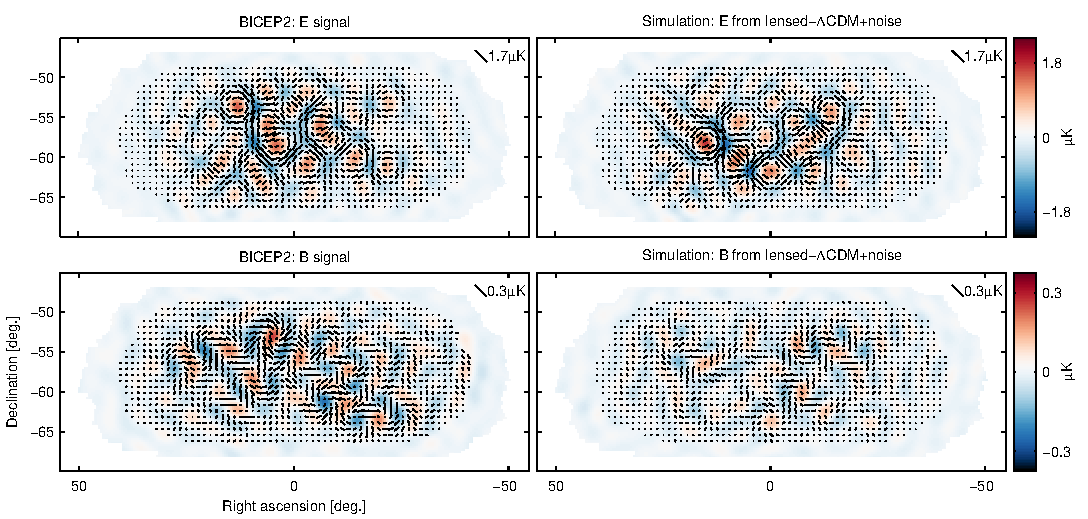
\includegraphics[width=\columnwidth]{eb_maps}
  \end{figure}
\end{frame}


\end{document}
